\documentclass[11pt]{article}

\usepackage[a4paper, margin=1in]{geometry}
\usepackage[T1]{fontenc}
\usepackage{lmodern}
\usepackage{microtype}
\usepackage{amsmath, amssymb, amsthm}
\usepackage{booktabs, tabularx}
\usepackage{enumitem}
\usepackage{xcolor}
\usepackage{listings}
\usepackage{algorithm}
\usepackage{algpseudocode}
\usepackage{tikz}
\usetikzlibrary{positioning, fit, arrows.meta, backgrounds}
\usepackage[numbers, sort&compress]{natbib}
\usepackage{hyperref}

\setlength{\emergencystretch}{3em}

\hypersetup{colorlinks=true, linkcolor=blue!50!black, citecolor=green!40!black, urlcolor=blue!60!black}

\newtheorem{theorem}{Theorem}
\newtheorem{proposition}[theorem]{Proposition}
\theoremstyle{definition}
\newtheorem{definition}{Definition}
\theoremstyle{remark}
\newtheorem{remark}{Remark}

\definecolor{codebg}{gray}{0.96}
\lstset{
  basicstyle=\ttfamily\footnotesize, backgroundcolor=\color{codebg}, frame=single,
  rulecolor=\color{gray!40}, columns=fullflexible, keepspaces=true, breaklines=true,
  keywordstyle=\color{blue!60!black}\bfseries, commentstyle=\color{green!40!black},
  morekeywords={fn, let, impl, pub, struct, enum, match, if, else, for, in, return, Ok, Err, Self, self, where, type, const}
}

\newcommand{\status}[1]{\textsc{#1}}
\newcommand{\impl}{\status{implemented}}
\newcommand{\partly}{\status{partial}}
\newcommand{\future}{\status{future work}}

\title{\textbf{Canggu}: A Quantum-Secure, MEV-Resistant Blockchain for Parallel Computing\\[4pt]
\large Version 2.0 --- Polkadot SDK Edition}

\author{\textit{Original design (v1.3):}\\ Dendi Suhubdy, Tejveer Singh, Mitul Dhawan, Maldini Sonkeng\\
\small Bitwyre~\cite{canggu-v13}\\[6pt]
\textit{Polkadot SDK edition (v2.0):}\\ Canggu contributors\\
\small \url{https://github.com/agustinustheo/canggu-blockchain}}

\date{October 25, 2026}

\begin{document}
\maketitle

\begin{abstract}
\noindent
Canggu is a layer-1 blockchain designed around four ideas: post-quantum account security, a
dependency-ordered (DAG) mempool that removes the cheapest forms of transaction reordering,
succinct zero-knowledge verification, and execution models that can exploit parallel hardware.
Version 1.3 of this whitepaper described those ideas as a from-scratch system. This version
specifies how Canggu is built on the Polkadot SDK (Substrate/FRAME), documents a working
reference implementation, and revisits the original design with measurements and a critical eye.
Concretely we implement (i) ML-DSA-65 (CRYSTALS-Dilithium, FIPS~204) account signatures verified
by a native host function; (ii) consensus-enforced cross-account transaction dependencies built on
the transaction pool's existing tag graph, together with the removal of fee tips as a priority
auction; (iii) on-chain Groth16 verification with an example ``private payroll'' circuit; and
(iv) a conflict-free batch-payment pallet. We correct several claims of v1.3: CRYSTALS-Kyber is a
key-encapsulation mechanism and cannot sign transactions, XMSS is a signature scheme rather than a
hash function, BLS12-381 SNARKs are \emph{not} quantum-resistant, and topological sorting does not
make MEV extraction computationally hard. Finally, we argue where GPUs belong in a Polkadot SDK
chain, which is behind deterministic host functions and in off-chain provers, not inside the state
transition function, and demonstrate it: batches of ML-DSA signatures are verified on an Apple
GPU through Metal, at up to $4.45\times$ the throughput of 12 CPU cores. A GPU validator and a
CPU validator stay in consensus over the same blocks.
\end{abstract}

\tableofcontents
\newpage

%=====================================================================
\section{Introduction}
%=====================================================================

Three pressures shape the next generation of blockchains. Large-scale quantum computers would break
the elliptic-curve signatures that protect almost every account today~\cite{shor1994,roetteler2017}.
Block producers routinely reorder, insert and censor transactions to extract value
(MEV)~\cite{flashboys}. And smart-contract platforms execute one transaction at a time on one core,
leaving most of a modern machine idle.

Canggu~\cite{canggu-v13} proposed answers to all three. The design, the name and the original
whitepaper are the work of the Bitwyre team listed above, who open-sourced it. This edition is an
independent rebuild of their idea. Its purpose is to explore how far the Polkadot SDK can be pushed
toward such a design, including onto GPUs, not to endorse every choice of the original, and it
says so where measurements disagree with v1.3. It makes the design concrete on
the Polkadot SDK~\cite{polkadotsdk}, a framework that already provides networking, a transaction
pool, block authoring and finality, a Wasm runtime with forkless upgrades, and the FRAME pallet
system. Building on it lets us focus on what is specific to Canggu, and every claim below is tied
to code that runs.

\paragraph{Contributions.}
\begin{enumerate}[leftmargin=*, itemsep=2pt]
  \item A post-quantum account model on Substrate: ML-DSA-65 signatures, accounts derived as
        $\mathsf{BLAKE2b\text{-}256}(pk)$, and verification through a native host function
        (\S\ref{sec:pq}).
  \item \texttt{CheckDagParents}, a transaction extension that turns the transaction pool into a
        cross-account dependency DAG and makes violating a dependency a consensus fault, plus a fee
        extension that removes tips (\S\ref{sec:dag}).
  \item A circuit-agnostic Groth16 verifier pallet backed by a native host function, and a private
        payroll circuit as a worked example (\S\ref{sec:zk}).
  \item A batch-payment pallet whose \emph{conflict-freedom contract} is what a parallel executor
        needs (\S\ref{sec:parallel}).
  \item An assessment of GPUs in a Polkadot SDK chain (\S\ref{sec:gpu}) and an honest list of
        what is not solved yet (\S\ref{sec:limits}).
\end{enumerate}

\paragraph{Status at a glance.} Table~\ref{tab:status} maps every component of v1.3 to its
Polkadot SDK realisation.

\begin{table}[ht]
\centering
\small
\begin{tabularx}{\textwidth}{@{}lXl@{}}
\toprule
\textbf{v1.3 component} & \textbf{Polkadot SDK realisation} & \textbf{Status} \\
\midrule
Dilithium signatures & \texttt{CangguSignature::MlDsa65}, host fn \texttt{ml\_dsa\_65\_verify} & \impl \\
Kyber key management & ML-KEM is a KEM, not a signature; reserved for encrypted mempool / transport & \future \\
XMSS ``hashing'' & BLAKE2b-256 for hashing; SLH-DSA (FIPS 205) as conservative signature option & \partly \\
Hybrid (classical + PQ) & Either-or crypto agility: classical variants kept for migration & \impl \\
DAG mempool & Pool \texttt{provides}/\texttt{requires} tags + \texttt{CheckDagParents} & \impl \\
MEV mitigation & Dependency enforcement, no tips, sealed order-then-reveal (\S\ref{sec:sealed}) & \partly \\
Tower BFT, rotating leader & Aura (round-robin slots, 2\,s) + GRANDPA finality & \impl \\
Sub-second finality & Tuned GRANDPA: 242\,ms p50 on localhost (\S\ref{sec:consensus}) & \partly \\
ZK-SNARK verification & \texttt{pallet-zk-verifier}: Groth16 and post-quantum SP1 STARKs (\S\ref{sec:sp1}) & \impl \\
Signature compression & One SP1 proof per intent batch replaces all keys and signatures (\S\ref{sec:sp1}) & \partly \\
GPU proof generation & Off-chain prover; GPU MSM/NTT back-ends (e.g.\ ICICLE) pluggable & \future \\
GPU acceleration & Batch ML-DSA verification on Apple Metal behind a host function & \impl \\
Parallel CPU/GPU contracts & Conflict-free batch payments; parallel executor & \partly \\
50{,}000+ TPS & Not supported by measurements with PQ signatures; see \S\ref{sec:eval} & \status{revised} \\
\bottomrule
\end{tabularx}
\caption{From the v1.3 design to the Polkadot SDK implementation.}
\label{tab:status}
\end{table}

%=====================================================================
\section{Problem Statement}
%=====================================================================

\begin{itemize}[leftmargin=*]
  \item \textbf{Quantum vulnerability.} ECDSA, EdDSA and Schnorr signatures (secp256k1, Ed25519,
        Sr25519) rely on the discrete-logarithm problem, which Shor's algorithm solves in polynomial
        time~\cite{shor1994}. Estimates put the break of a 256-bit curve at a few thousand logical
        qubits~\cite{roetteler2017}. Hash functions are only affected by Grover's
        algorithm~\cite{grover1996}, which halves their effective security.
  \item \textbf{MEV.} When a single party chooses transaction order, it can front-run, back-run and
        sandwich users. Fee-priority mempools make this an open auction~\cite{flashboys}.
  \item \textbf{Sequential execution.} Runtimes such as the EVM apply transactions one by one, even
        when they touch disjoint state.
  \item \textbf{Consensus bottlenecks.} Fast block production, fast finality and decentralisation
        pull in different directions.
\end{itemize}

%=====================================================================
\section{Architecture}
\label{sec:arch}
%=====================================================================

A Polkadot SDK chain has two halves. The \emph{node} (client) handles networking, the transaction
pool, consensus and storage, and is native code. The \emph{runtime} is the state transition function,
compiled to WebAssembly, stored on-chain and executed by every validator in a sandbox. The runtime
can only reach the outside world through \emph{host functions}, a fixed and versioned interface
the node implements. Figure~\ref{fig:arch} shows where each Canggu component lives.

\begin{figure}[ht]
\centering
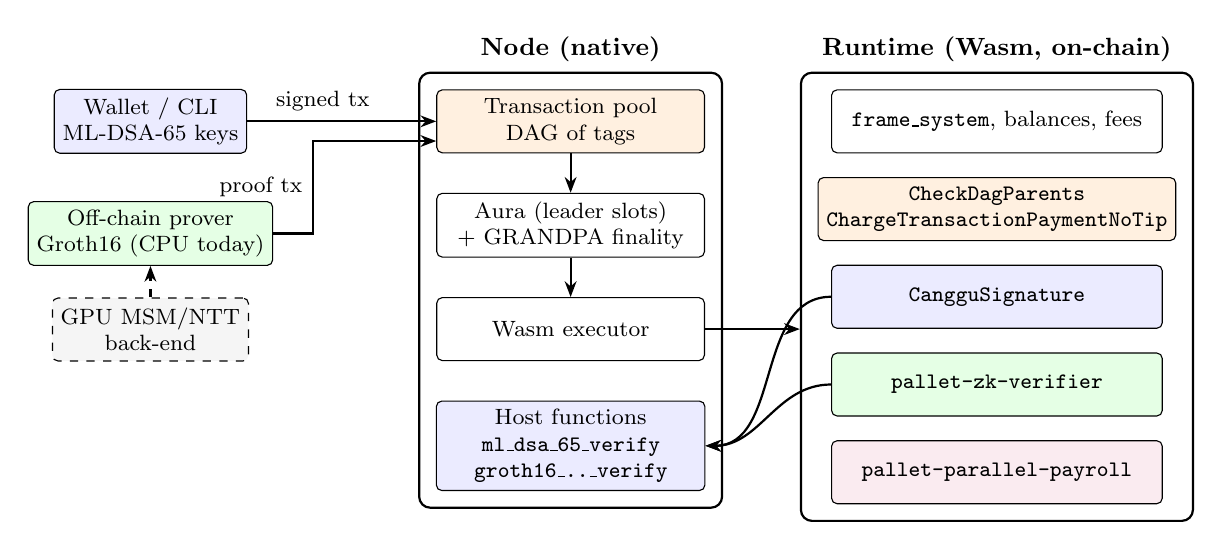
\begin{tikzpicture}[
  font=\footnotesize,
  box/.style={draw, rounded corners=2pt, align=center, minimum height=8mm, inner sep=3pt, fill=white},
  pq/.style={box, fill=blue!8}, dag/.style={box, fill=orange!12}, zk/.style={box, fill=green!10},
  par/.style={box, fill=purple!8}, fut/.style={box, dashed, fill=gray!8},
  arr/.style={-{Stealth[length=2mm]}, thick}, darr/.style={arr, dashed}
]
\node[pq] (wallet) {Wallet / CLI\\ML-DSA-65 keys};
\node[zk, below=6mm of wallet] (prover) {Off-chain prover\\Groth16 (CPU today)};
\node[fut, below=4mm of prover] (gpu) {GPU MSM/NTT\\back-end};

\node[dag, right=24mm of wallet, minimum width=34mm] (pool) {Transaction pool\\DAG of tags};
\node[box, below=5mm of pool, minimum width=34mm] (cons) {Aura (leader slots)\\+ GRANDPA finality};
\node[box, below=5mm of cons, minimum width=34mm] (exec) {Wasm executor};
\node[pq, below=5mm of exec, minimum width=34mm, text width=32mm] (host) {Host functions\\\texttt{ml\_dsa\_65\_verify}\\\texttt{groth16\_..\_verify}};
\begin{scope}[on background layer]
\node[draw, thick, rounded corners, fit=(pool)(cons)(exec)(host), inner sep=6pt, label={[font=\small\bfseries]above:Node (native)}] (node) {};
\end{scope}

\node[box, right=16mm of pool, minimum width=42mm] (sys) {\texttt{frame\_system}, balances, fees};
\node[dag, below=3mm of sys, minimum width=42mm] (ext) {\texttt{CheckDagParents}\\\texttt{ChargeTransactionPaymentNoTip}};
\node[pq, below=3mm of ext, minimum width=42mm] (sig) {\texttt{CangguSignature}};
\node[zk, below=3mm of sig, minimum width=42mm] (zkp) {\texttt{pallet-zk-verifier}};
\node[par, below=3mm of zkp, minimum width=42mm] (pay) {\texttt{pallet-parallel-payroll}};
\begin{scope}[on background layer]
\node[draw, thick, rounded corners, fit=(sys)(ext)(sig)(zkp)(pay), inner sep=6pt, label={[font=\small\bfseries]above:Runtime (Wasm, on-chain)}] (rt) {};
\end{scope}

\draw[arr] (wallet.east) -- node[above, pos=0.4]{signed tx} (wallet.east -| pool.west);
\draw[arr] (prover.east) -- ++(5mm,0) |- node[pos=0.25, left]{proof tx} ([yshift=-2.5mm]pool.west);
\draw[darr] (gpu) -- (prover);
\draw[arr] (pool) -- (cons);
\draw[arr] (cons) -- (exec);
\draw[arr] (exec.east) -- (rt.west |- exec.east);
\draw[arr] (sig.west) to[out=180, in=0] (host.east);
\draw[arr] (zkp.west) to[out=180, in=0] (host.east);
\end{tikzpicture}
\caption{Canggu on the Polkadot SDK. Expensive cryptography is pulled out of the Wasm runtime
into native host functions; that interface is also where hardware acceleration can be added without
touching consensus logic. Dashed: not yet implemented.}
\label{fig:arch}
\end{figure}

\paragraph{Transaction lifecycle.} A wallet signs a transaction with ML-DSA-65 and submits it to
any node. The pool validates it by calling into the runtime: the signature is checked by the
\texttt{ml\_dsa\_65\_verify} host function, \texttt{CheckNonce} and \texttt{CheckDagParents} emit its
\texttt{provides}/\texttt{requires} tags, and the no-tip fee extension checks it can pay. The
current Aura leader drains the pool in dependency order into a block. Every validator re-executes
the block, including the same extension checks, and GRANDPA finalises it.

%=====================================================================
\section{Post-Quantum Accounts}
\label{sec:pq}
%=====================================================================

\subsection{Choosing the primitives}

NIST finalised its first post-quantum standards in August 2024: ML-KEM (FIPS~203, formerly
CRYSTALS-Kyber)~\cite{fips203}, ML-DSA (FIPS~204, formerly CRYSTALS-Dilithium)~\cite{fips204} and
SLH-DSA (FIPS~205, formerly SPHINCS+)~\cite{fips205}. Version~1.3 proposed Kyber for ``key
management'', Dilithium for signing and XMSS for ``hashing''. Two corrections are needed:

\begin{itemize}[leftmargin=*]
  \item \textbf{ML-KEM cannot authenticate transactions.} A KEM establishes a shared secret between
        two parties; it has no signing operation. Account keys must be signature keys. In Canggu,
        ML-KEM is reserved for confidentiality: an encrypted mempool (\S\ref{sec:limits}) and
        hybrid key exchange in the peer-to-peer transport.
  \item \textbf{XMSS is a stateful signature scheme}~\cite{sp800208}, not a hash function, and
        reusing a one-time state is catastrophic. That makes it a poor fit for user wallets that
        may be restored on several devices. Transaction and block hashing in Canggu uses
        BLAKE2b-256. Grover's algorithm reduces its preimage resistance to $2^{128}$ quantum
        operations, which already meets the post-quantum target. Where a hash-based
        \emph{signature} is wanted for conservatism, the right choice is the stateless SLH-DSA.
\end{itemize}

Canggu therefore uses \textbf{ML-DSA-65} (NIST security category~3) for accounts. Public keys are
1{,}952 bytes and signatures 3{,}309 bytes.

\subsection{Account model}

Substrate identifies accounts by a 32-byte \texttt{AccountId32}, and a transaction carries the
signer's account plus a signature. For Ed25519 and Sr25519 the account \emph{is} the public key.
That cannot work for a 1{,}952-byte ML-DSA key, so Canggu defines
\[
  \mathsf{account}(pk) = \mathsf{BLAKE2b\text{-}256}(pk)
\]
and the signature variant carries the key itself:

\begin{lstlisting}
pub enum CangguSignature {
    Ed25519(ed25519::Signature),        // index 0  (transition period)
    Sr25519(sr25519::Signature),        // index 1  (transition period)
    Ecdsa(ecdsa::Signature),            // index 2  (transition period)
    MlDsa65 { public: MlDsa65Public, signature: MlDsa65Signature }, // index 3
}

impl Verify for CangguSignature {
    fn verify(&self, msg, signer: &AccountId32) -> bool {
        match self {
            Self::MlDsa65 { public, signature } =>
                public.to_account_id() == *signer
                    && canggu_crypto::ml_dsa_65_verify(&public.0, msg, &signature.0),
            /* classical variants as in sp_runtime::MultiSignature */
        }
    }
}
\end{lstlisting}

Binding the key to the account by hash prevents key substitution: a valid signature under a
different key fails the first check, at the cost of one hash. Signatures use the FIPS~204 context
string \texttt{"canggu/tx/v1"} for domain separation, and the payload is Substrate's standard signed
payload (call, extensions, spec and transaction version, genesis hash), so replay across chains and
runtime versions is prevented exactly as for classical accounts.

\subsection{Native verification through a host function}

Verification runs natively in the node through a new runtime interface, in the same way Substrate
verifies Sr25519:

\begin{lstlisting}
#[runtime_interface]
pub trait CangguCrypto {
    fn ml_dsa_65_verify(public: &[u8], msg: &[u8], signature: &[u8]) -> bool;
    fn groth16_bls12_381_verify(vk: &[u8], inputs: &[u8], proof: &[u8]) -> bool;
}
\end{lstlisting}

The node registers these functions alongside \texttt{sp\_io::SubstrateHostFunctions}. The
reference implementations use the pure-Rust \texttt{ml-dsa}~\cite{mldsarust} and
arkworks~\cite{arkworks} crates; ML-DSA-65 verification takes 61\,\textmu s (Table~\ref{tab:mldsa}).
Keeping the lattice and pairing arithmetic out of Wasm has two benefits. The node can use native
code, SIMD and later dedicated hardware, and the runtime does not have to ship and maintain the
cryptographic library. It also defines a narrow, deterministic contract (bytes in, one bit out)
that alternative implementations, including GPU ones, can meet (\S\ref{sec:gpu}).

\subsection{Transition period}

The classical variants keep existing wallets and tooling working during migration, which v1.3
called a ``hybrid'' period. We deliberately implement \emph{crypto agility} (each account picks
one scheme) rather than requiring both signatures on every transaction. A dual signature is only as
strong as its stronger half and costs the size of both. Once the ecosystem has migrated, a runtime
upgrade can reject the classical variants. Funds in classical accounts can then only be moved by
a final migration transaction or recovery process, which governance must schedule
\emph{before} a cryptographically relevant quantum computer exists.

\subsection{What is still classical}
Account signatures are only one of the places a chain uses elliptic curves. In the reference
implementation the Aura block-authoring keys (Sr25519), GRANDPA finality votes (Ed25519) and the
libp2p transport handshake (X25519) are still classical. A quantum adversary could therefore forge
blocks or finality votes even though user funds are protected. Migrating session keys to ML-DSA
requires keystore and consensus-engine support and is the top item on the roadmap.

%=====================================================================
\section{DAG-Ordered Transactions}
\label{sec:dag}
%=====================================================================

\subsection{The transaction pool is already a DAG}

Substrate's transaction pool does not keep a FIFO queue. Each validated transaction declares a set
of opaque \emph{tags} it \texttt{provides} and a set it \texttt{requires}. A transaction is
\emph{ready} when every required tag is provided by a transaction that is on-chain or already
ready. Otherwise it waits in the \emph{future} queue. Block authors drain the ready set in an order
consistent with these edges, which is Kahn's algorithm, as proposed in v1.3. The stock
\texttt{CheckNonce} extension uses this mechanism to chain one account's transactions: transaction
$(a, n)$ provides tag $\langle a, n\rangle$ and requires $\langle a, n-1\rangle$.

What is missing is the ability to depend on \emph{another account's} transaction, which is what
the v1.3 DEX example needs (``the user's swap references the current state of the pool via a parent
transaction'').

\subsection{\texttt{CheckDagParents}}

\begin{definition}
A transaction reference is a pair $(a, n)$ of an account and a nonce. Because nonces are consumed
exactly once and in order, $(a, n)$ identifies at most one transaction, and that transaction has
executed if and only if $\mathsf{nonce}(a) > n$ in the current state.
\end{definition}

\texttt{CheckDagParents} is a transaction extension carrying up to eight parent references:

\begin{algorithm}[ht]
\caption{\texttt{CheckDagParents} (pool validation and block execution)}
\begin{algorithmic}[1]
\Function{Validate}{$tx$, parents $P$}  \Comment{in the pool}
  \State $R \gets \{\, \mathsf{encode}(a, n) \mid (a,n) \in P,\ \mathsf{nonce}(a) \le n \,\}$
  \State \Return \textsc{Valid}(requires $=R$)  \Comment{same encoding as \texttt{CheckNonce}'s provides}
\EndFunction
\Function{Prepare}{$tx$, parents $P$} \Comment{when the block is executed}
  \If{$\exists (a,n)\in P: \mathsf{nonce}(a) \le n$}
     \State \Return \textsc{Invalid}(\textsc{Future})
  \EndIf
  \State \Return \textsc{Ok}
\EndFunction
\end{algorithmic}
\end{algorithm}

During validation, unmet parents become pool edges. During block execution the same condition is
re-checked against state. An author's block builder skips a transaction that fails it, and a block
that contains one is invalid and rejected by every honest validator. The extension runs before
\texttt{CheckNonce} in the extension pipeline, so a transaction rejected for a missing parent has
not mutated any state, including the sender's nonce.

\begin{theorem}[Dependency safety]
Assume account nonces are only incremented by \texttt{CheckNonce}. In any chain accepted by honest
validators, if transaction $t$ declares parent $(a, n)$, then the transaction $p$ signed by $a$ with
nonce $n$ is executed before $t$: in an earlier block, or earlier in the same block.
\end{theorem}
\begin{proof}
Honest validators execute every extrinsic of a block, and a block whose extrinsic fails
\textsc{Prepare} is invalid. So when $t$ executes, $\mathsf{nonce}(a) > n$. Nonces start at $0$ and
increase by exactly one when, and only when, $a$'s transaction with the current nonce is applied
(\texttt{CheckNonce} rejects any other nonce). Hence $a$'s transaction with nonce $n$ has been
applied, and it is $p$ by uniqueness.
\end{proof}

\noindent
The reference implementation checks this end to end (\S\ref{sec:eval}). A child submitted
\emph{before} its parent waits in the pool and is included only after the parent. Executing the
child first returns \textsc{Future}.

\subsection{Removing the priority auction}

In Substrate the fee extension also sets the transaction's \emph{priority}, which grows with its
tip. Tips are therefore a sealed-bid auction for position: the main tool an MEV searcher uses to
land in front of a victim. Canggu replaces \texttt{ChargeTransactionPayment} with
\texttt{ChargeTransactionPaymentNoTip}, which has an identical encoding but rejects any non-zero
tip. Priority then depends only on dispatch class, weight and length, never on payment.

\subsection{What a DAG does not do}
\label{sec:dag-limits}

Version~1.3 argued that MEV extraction becomes computationally infeasible because it requires
re-sorting a dense DAG in $\Omega(n^2)$ time. We do not rely on this argument:
\begin{enumerate}[leftmargin=*]
  \item A topological order is computed in $O(|V| + |E|)$, and the producer needs only \emph{one}
        profitable order, not all of them. Any linear extension of the DAG is a valid block, and
        their number is typically exponential, so the producer has more freedom than under
        nonce-only ordering, not less.
  \item Dependencies are declared by users. A victim's transaction that does not name a parent, and
        most do not, can be front-run by any transaction that is independent of it in the DAG.
  \item ``Hard to manipulate, easy to verify'' does not hold either. Checking that an order is
        topological is linear, and so is producing a manipulated one.
\end{enumerate}
What the DAG does provide is a \emph{safety} guarantee: dependencies that users state are enforced
by consensus. Combined with tip removal, this eliminates intra-dependency reordering and paid
priority. Mitigating front-running of independent transactions requires hiding transaction contents
until their order is fixed (\S\ref{sec:sealed}).

\subsection{Sealed ordering: order first, reveal later}
\label{sec:sealed}

The Rand Protocol whitepaper~\cite{rand}, also by Dendi Suhubdy, corrects the same mistake in its own
first draft. Hiding contents is not enough, because the party that orders can still order by
metadata (its Proposition~14.2). Its Theorem~15.4 eliminates front-running under three conditions:
(i) the order is fixed while contents are hidden; (ii) there is a single canonical order that binds
the block producer; (iii) what is visible before ordering is uniform. Rand meets (i) with $t$-of-$n$
threshold encryption~\cite{ferveo}. Practical schemes of that kind are pairing-based and not
post-quantum, and the running Rand chain does not implement it. Canggu's
\texttt{pallet-sealed-ordering} meets the three conditions with hash commitments:

\begin{enumerate}[leftmargin=*]
  \item \textbf{Commit} in block $N$: anyone, typically a relayer, posts
        \[ c = \mathsf{BLAKE2b}(\texttt{canggu/sealed/v1},\ \mathit{sender},\ \mathit{call},\
        \mathit{salt}) \]
        and locks a deposit. Commitments are uniform 32-byte values, and a relayer
        hides the sender (iii).
  \item \textbf{Reveal} in blocks $N{+}1 \dots N{+}w$: the sender publishes $(\mathit{call},
        \mathit{salt})$. Because $c$ binds the sender, nobody else can reveal or replay it.
  \item \textbf{Execute} at the start of block $N{+}w{+}1$: all revealed calls of block $N$ run in
        increasing order of $\mathsf{BLAKE2b}(c \,\|\, \mathsf{hash}(N))$ (ii). This order does not
        depend on inclusion or reveal order, and it cannot be computed when committing (i).
        Unrevealed commitments forfeit their deposit.
\end{enumerate}

\begin{proposition}
Let a victim's commitment be included in block $N$. Any transaction whose author learned the
victim's call from its reveal executes after the victim's call.
\end{proposition}
\begin{proof}
The reveal happens no earlier than block $N{+}1$, so a reacting commitment lands in a block
$N' > N$. Block $N'$ settles at $N'{+}w{+}1 > N{+}w{+}1$, after all of block $N$'s calls. Within
block $N$, every commitment was made without knowledge of the victim's call, and positions are
fixed by $\mathsf{hash}(N)$, which is unknown when committing.
\end{proof}

Compared with threshold encryption, commit-reveal concedes three things. A sender may decline to
reveal, a free option priced by the deposit. A leader may censor reveals within the window. The
leader of block $N$ can bias $\mathsf{hash}(N)$, though that only permutes commitments whose
contents nobody knows. Back-running is not addressed. On the dev chain, three senders revealed in
reverse order and executed in the canonical order, and an unrevealed commitment forfeited its
deposit. The pallet's tests check order independence and the proposition above. Anonymous
commitments without a relayer could use ring-membership proofs such as Parity's
\texttt{verifiable}~\cite{verifiable}, at the cost of reintroducing an elliptic-curve
assumption.

%=====================================================================
\section{Consensus}
\label{sec:consensus}
%=====================================================================

Version~1.3 called for a ``leader-verified consensus akin to Solana's Tower BFT''. Tower BFT is a
PBFT variant that uses Proof-of-History as a clock and exponentially growing vote
lockouts~\cite{solana2020whitepaper}. Canggu achieves the same split between fast leader-based
production and BFT finality with components that are proven in production:
\begin{itemize}[leftmargin=*]
  \item \textbf{Aura} assigns 2-second slots to authorities round-robin. The slot's leader authors
        the block, so leader rotation is deterministic and transparent.
  \item \textbf{GRANDPA}~\cite{grandpa} finalises chains rather than individual blocks. Validators
        vote on the highest block they consider final, and a supermajority ($>2/3$) finalises the
        chain up to that block.
\end{itemize}
With Substrate's defaults, blocks finalise about five seconds after they appear. Measurement shows
that this is not GRANDPA's message pattern but two conservative parameters. The voting rule
$\textsc{BeforeBestBlockBy}(2)$ makes validators vote two blocks behind the best block, which costs
two slot times. A voter also waits up to $2g$ before prevoting and $4g$ before precommitting, where
$g$ is the gossip duration (333\,ms by default). Lowering the vote lag does not affect safety: a
block is final only with precommits from more than two-thirds of the voters, and votes for a
losing fork finalise the common ancestor instead. Both parameters are exposed as node flags, and
the slot length as a compile-time constant.

\begin{table}[ht]
\centering\small
\begin{tabular}{@{}rrrrr@{}}
\toprule
\textbf{Slot} & \textbf{Gossip $g$} & \textbf{Vote lag} & \textbf{Finality p50} & \textbf{p90} \\
\midrule
2\,s   & 333\,ms & 2 & 5\,s     & 6\,s \\
2\,s   & 333\,ms & 0 & 1\,s     & 2\,s \\
2\,s   & 50\,ms  & 0 & 242\,ms  & 288\,ms \\
500\,ms & 333\,ms & 2 & 2\,s    & 3\,s \\
500\,ms & 50\,ms & 0 & 217\,ms  & 293\,ms \\
500\,ms & 25\,ms & 0 & 121\,ms  & 173\,ms \\
\bottomrule
\end{tabular}
\caption{Time from a block's first appearance to its finalisation, two validators on localhost.}
\label{tab:finality}
\end{table}

Table~\ref{tab:finality} is a lower bound: on localhost messages arrive almost instantly. Over a
real network $g$ must exceed the message delay between validators, and each round needs about two
delays. A validator set with 50--100\,ms between members should therefore finalise in well under a
second, while a globally distributed one probably will not. v1.3's sub-second claim is reachable
with GRANDPA for a geographically compact validator set, and remains to be measured over a real
network.

Running as a Polkadot parachain or JAM service~\cite{graypaper} instead would buy shared security,
at the cost of relay-chain finality latency. It would also cost Canggu its custom host functions
(\S\ref{sec:pq}, \S\ref{sec:metal}): relay-chain validators re-execute parachain blocks with
Polkadot's standard host interface, so ML-DSA and proof verification would have to run inside the
runtime, and the GPU back-end would not apply.

%=====================================================================
\section{Zero-Knowledge Verification}
\label{sec:zk}
%=====================================================================

\subsection{Prover/verifier split}
Proof generation runs off-chain on any hardware. The chain only verifies. \texttt{pallet-zk-verifier}
is circuit-agnostic:
\begin{itemize}[leftmargin=*]
  \item \texttt{register\_verifying\_key(vk)} stores a Groth16/BLS12-381 verifying key under
        $\mathsf{id} = \mathsf{BLAKE2b}(vk)$.
  \item \texttt{submit\_proof(id, inputs, proof)} calls the \texttt{groth16\_bls12\_381\_verify}
        host function and, on success, records the statement $\mathsf{BLAKE2b}(\mathsf{id}\,\|\,
        \mathsf{inputs})$ so other pallets and off-chain consumers can rely on it.
\end{itemize}
Malformed keys, proofs and non-canonical field elements make the host function return
\texttt{false} rather than panic. A failed verification still pays its full fee.

Verification cost is independent of circuit size: three pairings (the fourth,
$e(\alpha,\beta)$, is precomputed) and a multi-scalar multiplication over the $\ell$ public inputs.
It is therefore $O(\ell)$, which v1.3 called ``$O(1)$''. The two agree for the small, fixed $\ell$
of a given circuit.

\subsection{Example: private payroll commitment}

The bundled circuit connects ZK to Canggu's payroll use case. For a fixed number of recipients $N$,
it proves
\[
\exists\, s, a_1, \dots, a_N:\quad a_i \in [0, 2^{64}),\quad \sum_i a_i = T,\quad
\mathsf{MiMC\text{-}MP}(s, a_1,\dots,a_N) = C
\]
for public $(T, C)$. An employer publishes the commitment $C$ to a salary table and later proves
that the payroll it funds totals $T$, without revealing any salary. The commitment uses
MiMC~\cite{mimc} with exponent $5$ (a permutation of the BLS12-381 scalar field, since
$\gcd(5, r-1)=1$), 110 rounds, in Miyaguchi--Preneel mode. Each round costs three R1CS constraints,
each range check $64$, and materialising each amount and each intermediate hash one more, so the
circuit has
\[
330\,(N+1) + 64N + N + (N+1) + 2 \;=\; 396N + 333
\]
constraints, e.g.\ 1{,}917 for $N = 4$ (Table~\ref{tab:zk}). This is demonstration code: the hash parameters are
standard but the implementation has not been audited.

\subsection{Security notes and corrections}
\begin{itemize}[leftmargin=*]
  \item \textbf{Trusted setup.} Groth16 needs a circuit-specific setup whose randomness (``toxic
        waste'') allows forging proofs. The CLI performs a single-party setup for demonstration.
        Production keys require a multi-party ceremony, which is secure if one participant is honest.
  \item \textbf{BLS12-381 is not post-quantum.} Version~1.3 described ``quantum-resistant curves
        (e.g.\ BLS12-381 with NIST-approved tweaks)''. No such tweak exists. Pairing-based SNARKs rely
        on discrete logarithms in groups of roughly 255 bits, which Shor's algorithm breaks. A
        quantum adversary could \emph{forge} Groth16 proofs, although Groth16's perfect
        zero-knowledge means it could not extract witnesses from existing proofs. The post-quantum
        path is hash-based proof systems (STARKs/FRI~\cite{starks}), and Canggu now has one
        (\S\ref{sec:sp1}).
\end{itemize}

\subsection{Post-quantum proofs and signature compression with SP1}
\label{sec:sp1}

SP1~\cite{sp1} proves the execution of ordinary Rust programs compiled to RISC-V. Its
\emph{compressed} proofs are STARKs over the KoalaBear field with Poseidon2 Merkle commitments and
FRI. They use no pairings or elliptic curves, rely only on hash functions, and need no trusted
setup. Canggu verifies them with one more host function, \texttt{sp1\_v6\_verify\_compressed}.
SP1's verifier does not build for the \texttt{wasm32v1-none} target that Polkadot SDK runtimes
use. Two programs use it:

\begin{itemize}[leftmargin=*]
  \item \textbf{Payroll.} The statement of \S\ref{sec:zk} written as a short Rust function,
        with a Keccak commitment instead of MiMC. \texttt{pallet-zk-verifier} accepts its proofs
        next to Groth16 and records the statement $(\mathit{program}, \mathit{public\ values})$.
  \item \textbf{Signature compression.} An ML-DSA-65 verifier runs inside SP1 with Keccak-f
        delegated to SP1's precompile. It is bit-exact with the RustCrypto implementation on 4{,}280
        native cases and 460 zkVM executions. It proves that every $(pk_i, m_i, \sigma_i)$ in a
        batch is valid and commits
        \[
          n \,\|\, \mathsf{Keccak}(\mathit{ctx}) \,\|\, \mathsf{Keccak}\Bigl(\textstyle\big\|_i\,
          \mathsf{BLAKE2b}(pk_i) \,\|\, \mathsf{Keccak}(m_i)\Bigr).
        \]
        \texttt{pallet-pq-intents::submit\_compressed} receives only $(\mathit{sender}_i,
        \mathit{intent}_i)$ pairs and the proof. Because accounts are $\mathsf{BLAKE2b}(pk)$, the
        runtime can rebuild the committed value from the intents and the genesis hash alone, so
        the proof binds exactly these senders and intents on this chain. No key or signature
        reaches the block.
\end{itemize}

\begin{table}[ht]
\centering\small
\begin{tabular}{@{}lr@{}}
\toprule
Proof size (any program, any batch) & 1{,}272{,}546\,B \\
Verification (native / through the node's host function) & 25.5\,ms / $\approx$40\,ms \\
ML-DSA-65 inside SP1 (with / without Keccak precompile) & 0.70\,M / 1.83\,M cycles \\
Proving \texttt{mldsa-batch}, 4 / 64 / 128 signatures & 72\,s / 617\,s / 1{,}219\,s \\
Peak memory while proving & 15--17\,GB \\
Break-even against raw keys and signatures & $\approx$242 signatures ($\approx$37\,min) \\
Proving \texttt{payroll}, 16 / 65{,}536 amounts & 50\,s / 141\,s \\
\bottomrule
\end{tabular}
\caption{SP1 v6.10 on an Apple M4 Pro, CPU prover. Live on a development chain, a five-salary
payroll proof took 59\,s and an eight-intent compressed batch 113\,s to prove. Both verified on
chain.}
\label{tab:sp1}
\end{table}

Table~\ref{tab:sp1} gives the economics. A compressed proof costs as much block space as
$\approx$242 ML-DSA keys and signatures, and the CPU prover spends $\approx$9.4\,s per signature.
Compression therefore works end to end but is a net loss on a laptop: the eight-intent demonstration
batch is 30 times larger than the signatures it replaces. It pays off for batches of hundreds of
signatures proven on GPUs (SP1's GPU prover targets CUDA), which is the regime Rand Protocol's
pipelined aggregator market~\cite{rand} is designed for. Two findings matter for any chain adopting
SP1. First, the raw verifier accepts several byte strings for one valid proof: it ignores trailing
bytes and silently reduces field elements $\geq p$. Canggu's wrapper accepts only the canonical
encoding, which matters for anything that hashes or deduplicates proofs. Second, SP1's default
prover settings exceeded 33\,GB of memory at 16 signatures, so a memory-safe configuration
is part of the tooling.

%=====================================================================
\section{Parallel Execution}
\label{sec:parallel}
%=====================================================================

\subsection{The payroll pallet}

Version~1.3's flagship example is a payroll: the CPU validates and debits the employer once, and
the GPU credits all employees ``in parallel''. \texttt{pallet-parallel-payroll} implements the
semantics and, more importantly, the \emph{conflict-freedom contract} that makes parallel execution
legal:

\begin{algorithm}[ht]
\caption{\texttt{batch\_pay}$(\mathit{payer}, [(r_1, v_1), \dots, (r_N, v_N)])$}
\begin{algorithmic}[1]
\State \textbf{require} $r_i$ pairwise distinct and $\mathit{payer} \notin \{r_i\}$ \Comment{disjoint write sets}
\State $V \gets \sum_i v_i$ (checked) \Comment{phase 1: sequential}
\State $c \gets \textsc{Withdraw}(\mathit{payer}, V)$ \Comment{one balance check, one debit}
\ForAll{$i$} \Comment{phase 2: data-parallel}
  \State $(c_i, c) \gets \textsc{Split}(c, v_i)$;\ \ \textsc{Resolve}$(r_i, c_i)$
\EndFor
\end{algorithmic}
\end{algorithm}

\begin{proposition}
Under the precondition of line~1, the credits of phase~2 commute: every permutation yields the same
post-state. The call is atomic (all credits or none) and conserves total issuance.
\end{proposition}
\begin{proof}[Proof sketch]
Credit $i$ reads and writes only $r_i$'s account, and the accounts are pairwise distinct and distinct
from the payer, so the operations act on disjoint state and commute. Dispatch is transactional, so
any failing credit reverts the whole call. The withdrawn imbalance is split exactly into the credits,
so no value is created or destroyed. All three properties are covered by the pallet's tests.
\end{proof}

Today the credits are applied in a loop. The runtime is single-threaded Wasm, and each credit is
dominated by state-trie reads and writes. The pallet nonetheless guarantees what a parallel executor
needs: transactions or sub-operations with \emph{declared, disjoint access sets}.

\subsection{Weights}
Weights must reflect execution time on reference hardware, because they bound block production time.
Version~1.3's ``parallel gas'' per GPU thread block is only meaningful once execution actually runs in
parallel and its cost has been measured. Until then Canggu charges linear weights for batch payments.
All weights in the reference implementation are hand-set and must be replaced by benchmarks before
production.

%=====================================================================
\section{GPUs and the Polkadot SDK}
\label{sec:gpu}
%=====================================================================

Can the Polkadot SDK run on GPUs? The useful answer separates the parts of a node.

\paragraph{Not in the state transition function.} Every validator must compute bit-identical state
roots, so the runtime has to be deterministic, metered and sandboxed. GPU execution fails all three
as a general contract platform. Floating point and the order of reductions vary across vendors,
drivers and architectures. Kernels cannot be pre-empted or metered per instruction, so gas
accounting has no hook. Kernels cannot reach the Merkle-trie state, so every storage access would be
a host round-trip. Requiring CUDA would also make one vendor's hardware a consensus dependency and
exclude CPU-only validators that must re-execute blocks. The v1.3 claim that 10{,}000 stablecoin
transfers run ``in under 1\,ms'' on a GPU ignores that the work is updating 10{,}000 trie leaves,
not adding 10{,}000 integers.

\paragraph{Behind host functions: yes, with a contract.} A host function is a pure function from
bytes to bytes with a CPU reference implementation. A node may compute it on a GPU if it returns
\emph{exactly} the same output, which is achievable for integer-only kernels. Good candidates are
batch ML-DSA verification (dominated by number-theoretic transforms), multi-scalar multiplication
and NTTs for SNARK/STARK verification, and bulk hashing. The deployment discipline is: a CPU
reference implementation defines consensus, the GPU back-end is differentially tested against it,
and nodes without a GPU fall back to the CPU. Canggu's \texttt{canggu\_crypto} interface is designed
for this, and \S\ref{sec:metal} implements it.

\paragraph{Off-chain proving: the best fit.} Proof generation is dominated by MSMs and FFTs that
parallelise extremely well, and its output is checked on-chain, so it does not have to be
deterministic. GPU libraries such as ICICLE~\cite{icicle} report order-of-magnitude speed-ups for
these kernels. This is also how GPUs can raise Canggu's throughput under post-quantum signatures:
a GPU prover can aggregate thousands of ML-DSA signatures into one STARK, so blocks carry one proof
instead of 3.3\,kB per transaction (\S\ref{sec:eval}).

\paragraph{Parallel execution: multi-core first.} Parallelism inside block execution is a CPU
problem: run conflict-free transactions on different cores, using declared access sets such as
those of the payroll pallet. JAM~\cite{graypaper} takes this further with many independent cores
executing PolkaVM code in parallel.

\subsection{A Metal implementation}
\label{sec:metal}

To test how close a Polkadot SDK chain can get to the GPU, Canggu adds a batch host function,
\[
\texttt{ml\_dsa\_65\_batch\_verify}\colon [(pk_i, m_i, \sigma_i)]_{i=1}^{n} \mapsto [b_i]_{i=1}^{n},
\]
and a consumer for it. In \texttt{pallet-pq-intents}, users sign transfer \emph{intents} off-chain
and a relayer submits up to 640 of them in one extrinsic. The runtime makes a single host call per
batch, then executes or rejects each intent independently. The node chooses at start-up where the
call runs: one CPU core (the reference that defines the verdicts), all cores, or an Apple GPU via
Metal (\texttt{--crypto-backend metal}).

\paragraph{Kernels.} FIPS~204 verification is split at the point where work becomes fixed-size and
data-parallel. A multi-threaded CPU stage decodes keys and signatures, checks hint encodings and the
$\|z\|_\infty$ bound, and computes $tr$, $\mu$ and the challenge $c$. Four integer-only Metal kernels
then compute the input NTTs, the matrix expansion fused with $\hat{A}\hat{z}$ (the dominant cost:
30 SHAKE128 rejection-sampled polynomials per signature), the inverse NTT with UseHint and
$w_1$ encoding, and the final SHAKE256 comparison with $\tilde{c}$. Small batches below 64
signatures go to the CPU, because a GPU submission has a fixed latency of about 0.2\,ms.

\paragraph{Bit-exactness.} A GPU that disagreed with the CPU on a single signature would fork its
validator off the network, so correctness is established three ways:
\begin{itemize}[leftmargin=*]
  \item \emph{Differential tests.} The Metal kernels, a pure-Rust mirror of each kernel, and the
        RustCrypto \texttt{ml-dsa} crate are compared on 5{,}454 items: 2{,}504 valid signatures,
        and 2{,}950 corrupted ones (bit flips in every field, malformed hints, $z$ at the bound,
        wrong contexts and lengths). All three agree on every item, both as one batch and as
        random sub-batches.
  \item \emph{Self-test.} At node start-up the GPU's UseHint is checked against the CPU for
        \emph{every} input below $q$, along with the modular arithmetic and Keccak-f. During
        development this caught a deliberately planted off-by-one that no real signature
        exercises.
  \item \emph{Consensus.} Two validators run with different backends, Metal and a single CPU core.
        Aura alternates authors, so each batch is verified on the GPU by one validator and on the
        CPU by the other. Six blocks of 256 intents each, with forgeries included, were authored
        alternately by both validators and finalised. Both nodes report identical hashes for every
        block.
\end{itemize}

\begin{table}[ht]
\centering\small
\begin{tabular}{@{}rrrrrr@{}}
\toprule
\textbf{Batch} & \textbf{ml-dsa, 1 core} & \textbf{ml-dsa, 12 cores} & \textbf{Metal (wall)} & \textbf{GPU busy} & \textbf{vs 12 cores} \\
\midrule
1    & 0.060\,ms & 0.060\,ms & 0.330\,ms & 0.203\,ms & $0.18\times$ \\
64   & 3.77\,ms  & 0.61\,ms  & 0.45\,ms  & 0.23\,ms  & $1.35\times$ \\
256  & 15.2\,ms  & 1.95\,ms  & 0.85\,ms  & 0.43\,ms  & $2.29\times$ \\
1024 & 61.2\,ms  & 7.52\,ms  & 2.12\,ms  & 1.50\,ms  & $3.55\times$ \\
4096 & 246\,ms   & 29.0\,ms  & 6.51\,ms  & 5.59\,ms  & $4.45\times$ \\
\bottomrule
\end{tabular}
\caption{Batch ML-DSA-65 verification on an Apple M4 Pro (medians). Metal wall time includes the
CPU stage and buffer transfers; GPU busy time is reported by Metal's command-buffer timestamps.
At 4{,}096 signatures the GPU verifies 630k signatures per second, 1.37\,\textmu s of GPU time each.}
\label{tab:metal}
\end{table}

\paragraph{Assessment.} The GPU wins for batches of 64 signatures and more, and the advantage
grows with batch size (Table~\ref{tab:metal}). Inside a live node, 640 signatures took 8.4\,ms of
wall time and 4.1\,ms of GPU time. That is slower than the warm benchmark, because the batch is
copied across the host-function boundary and the GPU was shared with other processes. Weights are
still charged at single-core CPU cost, because every validator, GPU or not, must keep up. The GPU
therefore buys headroom and lower block-execution latency, not a higher on-chain limit, unless the
validator set agrees to assume GPU hardware. Only Metal is implemented. A CUDA back-end would sit
behind the same interface and the same differential tests.

%=====================================================================
\section{Implementation and Evaluation}
\label{sec:eval}
%=====================================================================

\subsection{Implementation}
The reference implementation targets \texttt{polkadot-stable2609} and Rust~1.93.

\begin{table}[ht]
\centering\small
\begin{tabularx}{\textwidth}{@{}lX@{}}
\toprule
\textbf{Crate} & \textbf{Role} \\
\midrule
\texttt{canggu-primitives} & \texttt{CangguSignature}, \texttt{CangguSigner}, host functions, dev keyring \\
\texttt{canggu-dag-ordering} & \texttt{CheckDagParents}, \texttt{ChargeTransactionPaymentNoTip} \\
\texttt{pallet-zk-verifier} & Groth16 verifying-key registry and proof verification \\
\texttt{pallet-parallel-payroll} & Conflict-free batch payments \\
\texttt{canggu-zk} & Private payroll circuit, setup and proving (off-chain) \\
\texttt{pallet-pq-intents} & Batches of ML-DSA-signed intents, one batch host call \\
\texttt{canggu-gpu} & ML-DSA-65 batch verification on Metal, CPU mirror, differential tests \\
\texttt{canggu-runtime} & FRAME runtime wiring all of the above \\
\texttt{canggu-node} & Aura + GRANDPA node with Canggu host functions \\
\texttt{canggu-cli} & ML-DSA wallet, prover, end-to-end demo, benchmarks \\
\bottomrule
\end{tabularx}
\caption{Crates of the reference implementation.}
\end{table}

\noindent Unit tests cover each pallet and extension. Runtime integration tests push ML-DSA-signed
extrinsics through \texttt{Executive}: valid transfers execute, bit-flipped and key-substituted
signatures are rejected with \textsc{BadProof}, a child applied before its parent returns
\textsc{Future}, and tips are refused. The CLI's \texttt{demo} command repeats these checks against
a live development node.

\subsection{Measurements}
\label{sec:measure}
All numbers were taken on an Apple M4 Pro (12 cores) with release builds.

% Generated from `canggu bench --recipients 4,16,64,256,1024` and the end-to-end demo
% (Apple M4 Pro, 12 cores, release build, polkadot-stable2609).

\begin{table}[ht]
\centering\small
\begin{tabular}{@{}lrr@{}}
\toprule
\textbf{ML-DSA-65 (pure Rust, one core)} & & \\
\midrule
Sign (deterministic) & \multicolumn{2}{r}{$\approx 0.75$\,ms} \\
Verify (host function reference implementation) & \multicolumn{2}{r}{61\,\textmu s} \\
Public key / signature & \multicolumn{2}{r}{1{,}952\,B / 3{,}309\,B} \\
Signed \texttt{transfer\_keep\_alive} extrinsic & \multicolumn{2}{r}{5{,}345\,B} \\
\bottomrule
\end{tabular}
\caption{Post-quantum account costs.}
\label{tab:mldsa}
\end{table}

\begin{table}[ht]
\centering\small
\begin{tabular}{@{}rrrrrr@{}}
\toprule
\textbf{Recipients $N$} & \textbf{Constraints} & \textbf{Setup} & \textbf{Prove} & \textbf{Verify} & \textbf{Proof} \\
\midrule
4    & 1{,}917   & 25\,ms  & 33\,ms  & 2.5\,ms & 192\,B \\
16   & 6{,}669   & 57\,ms  & 68\,ms  & 2.3\,ms & 192\,B \\
64   & 25{,}677  & 176\,ms & 185\,ms & 2.3\,ms & 192\,B \\
256  & 101{,}709 & 0.60\,s & 0.57\,s & 2.3\,ms & 192\,B \\
1024 & 405{,}837 & 2.3\,s  & 2.0\,s  & 2.3\,ms & 192\,B \\
\bottomrule
\end{tabular}
\caption{Private payroll circuit, Groth16 over BLS12-381 (arkworks). Setup and proving use all
cores on the CPU; verification is the single-threaded host function and includes decoding and
subgroup-checking the verifying key. Proving cost grows linearly with $N$; verification does not.}
\label{tab:zk}
\end{table}

\noindent
Two observations matter for the design. First, the prover/verifier asymmetry is real and large:
at $N = 1024$ proving takes $\sim 870\times$ longer than verifying (on 12 cores versus one), and every validator only
pays the verifier's 2.3\,ms. Second, a careless circuit can scale quadratically. An early version
of the gadget kept the running hash as a symbolic linear combination, so every MiMC round re-copied
its whole history, and proving $N = 256$ took 119\,s instead of 0.57\,s. Materialising the hash
state and each amount as a witness costs one constraint each and restores linear scaling.

\paragraph{Capacity of the current configuration.} A block may contain up to 5\,MiB, of which 75\,\%
is available to normal transactions, and 1\,s of execution weight in a 2\,s slot. With 5.3\,kB per
ML-DSA transfer, a block holds about 740 transfers, so the chain is \emph{bandwidth-bound} at roughly
370 transfers per second. Signature verification for those transfers takes about
$740 \times 61\,\text{\textmu s} \approx 45$\,ms on one core, far from the weight limit.


\subsection{Throughput, revisited}
An ML-DSA-65 transfer is 5{,}345 bytes on the wire, against roughly 150\,bytes for an Sr25519
transfer. The current configuration is bandwidth-bound at about 370 transfers per second
(\S\ref{sec:measure}). At v1.3's target of 50{,}000\,TPS the chain would have to gossip, store and
verify about 265\,MB/s of transaction data, before any other overhead. Signature verification itself parallelises across
cores and is not the binding constraint. Bandwidth and storage are. We therefore no longer claim
50{,}000\,TPS. Reaching that order of magnitude with post-quantum signatures requires
\emph{signature compression}: the leader, or a GPU prover, verifies the block's signatures inside a
STARK and replaces them with one proof. This is the strongest argument for the ZK pillar.
\S\ref{sec:sp1} implements it per intent batch and measures the price: a 1.27\,MB proof, so
compression saves space only above $\approx$242 signatures, and minutes to hours of proving
unless GPUs do it.

%=====================================================================
\section{Limitations and Roadmap}
\label{sec:limits}
%=====================================================================

\begin{enumerate}[leftmargin=*]
  \item \textbf{Post-quantum consensus keys.} Move Aura and GRANDPA session keys to ML-DSA. This
        needs keystore support, larger votes and justifications, and is a prerequisite for
        calling the chain, not only its accounts, quantum-secure.
  \item \textbf{Threshold-encrypted mempool.} Replace commit--reveal (\S\ref{sec:sealed}) with
        encryption to a validator threshold key, which removes the free option and needs no
        second transaction. Post-quantum threshold decryption is still a research topic;
        order-fairness protocols~\cite{aequitas} are an alternative.
  \item \textbf{Post-quantum proofs.} Done with SP1 (\S\ref{sec:sp1}). Retire the Groth16 path and
        pin the verifier version through host-function versioning.
  \item \textbf{Windowed signature compression.} Per-batch compression works
        (\S\ref{sec:sp1}); scale it with Rand's block-level aggregation~\cite{rand}: GPU aggregators prove a STARK over the ML-DSA verifications of a
        window of finalised blocks off the critical path, the aggregate that covers the most wins,
        and proofs are bound to their aggregator.
  \item \textbf{More GPU back-ends.} CUDA next to Metal (\S\ref{sec:metal}), and GPU Groth16/STARK
        verification behind the same differential-testing discipline.
  \item \textbf{Parallel block execution} using declared access sets.
  \item \textbf{Benchmarked weights}, a multi-party trusted setup ceremony, and audits.
  \item \textbf{Retire classical account signatures} by runtime upgrade.
\end{enumerate}

%=====================================================================
\section{Conclusion}
%=====================================================================

Building Canggu on the Polkadot SDK shows that most of its vision fits naturally into an existing,
production-grade framework. Post-quantum accounts are a new signature type and a host function.
The DAG mempool is a transaction extension on top of a pool that already orders by dependencies.
On-chain SNARK verification is a pallet and a host function. Bringing the design into contact with
code and measurements also sharpened it. Several v1.3 claims did not survive, among them
Kyber-signed wallets, quantum-safe BLS12-381 and MEV resistance through graph complexity. Others
became more precise: GPUs belong in provers and behind deterministic host functions, and the ZK
pillar is what can make post-quantum signatures affordable at scale.

\bibliographystyle{plainnat}
\bibliography{references}

\appendix
\section{Corrections to Version 1.3}

\begin{table}[ht]
\centering\small
\begin{tabularx}{\textwidth}{@{}XX@{}}
\toprule
\textbf{v1.3 statement} & \textbf{Correction} \\
\midrule
Users generate key pairs with Kyber for wallet operations. & ML-KEM is a KEM. Wallet keys are ML-DSA (FIPS 204). \\
Transactions are hashed with XMSS. & XMSS is a stateful signature scheme. Hashing uses BLAKE2b-256 (128-bit post-quantum preimage security). \\
ZK-SNARKs on ``quantum-resistant curves (e.g.\ BLS12-381)''. & Pairing-based SNARKs are broken by Shor's algorithm. Use STARKs for post-quantum soundness. \\
DAG reordering costs $\Omega(n^2)$, making MEV infeasible. & Topological sorting is $O(|V|+|E|)$ and any linear extension is valid. DAGs enforce declared dependencies only. \\
FIFO sorting is $O(n)$ / $O(n \log n)$ (both stated). & Neither is relevant: Substrate pools order by priority and tags. \\
Groth16 verification is $O(1)$. & $O(\ell)$ in the number of public inputs, independent of circuit size. \\
Solana executes transactions sequentially in a single thread. & Solana's Sealevel executes non-conflicting transactions in parallel. Canggu's distinction is GPU acceleration, not parallelism as such. \\
50{,}000+ TPS with Dilithium signatures. & Not supported. Requires signature compression (\S\ref{sec:eval}). \\
Sub-second finality with Tower-BFT-style consensus. & Aura + GRANDPA does it once the vote lag and gossip duration are tuned (localhost measurement; network latency pending). \\
\bottomrule
\end{tabularx}
\end{table}

\end{document}
